\documentclass[a4paper,11pt,twoside]{article}
\usepackage{styleN7_utf8}


%----- commandes locales %--------------------------------------------------


%====[ PAGE DE TITRE ]======================================================
\title{Manuscrit manager}
\renewcommand{\and}{\hspace{1em}}
\author{Inès Carrasco \and Marie Elisabelar \and Florent Fayollas\\
		Aurélie Forzani \and Mariem Jridi \and Nicolas Urien}
\subject{Manuel de l'utilisateur (version 1)}
\date{2016~--~2017}
\discipline{Technologie Objet}
\promotion{ENSEEIHT --- 1\iere~Année Informatique}


%====[ DEBUT DU DOCUMENT ]==================================================
\begin{document}
\maketitle
\newpage

%---------------%------------------------------ corps du document
\section{Objectif général du projet}
Le ``Manuscrit Manager'', sera une application puissante, qui permettra l'écriture des ouvrages d'une manière plus sophistiquée qu'un simple traitement de texte. En effet, si l'utilisateur manque d'inspiration, qu'il cherche à rajouter un nouveau personnage, qu'il ne peut pas organiser ses idées ni se repérer facilement dans ce qu'il a écrit,\ldots il pourra utiliser ce programme.

Le ``Manuscrit Manager'' sera le programme qui offrira toutes ces opportunités aux utilisateurs. En facilitant toutes ces tâches, il augmentera la productivité de l'utilisateur et accélérera le temps de production de son ouvrage.


%%%%%%%%%%%%%%%%%%%%%%%%%%%%%%%%%%%%%%%%%%%%%%%%%%%%%%%%%%%%%%%%%%%%%%%%%%%%%%%%%%%%%%%%%%%%%%%%%%%%%%%%%%%%%%%%%%%%%
%%%%%%%%%%%%%%%%%%%%%%%%%%%%%%%%%%%%%%%%%%%%%%%%%%%%%%%%%%%%%%%%%%%%%%%%%%%%%%%%%%%%%%%%%%%%%%%%%%%%%%%%%%%%%%%%%%%%%
\section{Fonctionnalités de l'application}
L'application en tant que telle est découpée en modules ayant chacun une fonction précise~:
\begin{itemize}
	\item Saisie de texte augmentée~;
    \item Ressources d'écriture~;
    \item Carte mentale (schéma permettant de visualiser les liens existant entre différents éléments)~;
    \item Gestion de l'univers spatio-temporel~;
    \item Gestion de personnages~;
    \item Et sauvegarde et chargement d'un projet.
\end{itemize}


%%%%%%%%%%%%%%%%%%%%%%%%%%%%%%%%%%%%%%%%%%%%%%%%%%%%%%%%%%%%%%%
\subsection{Saisie de texte augmentée}
La toute première fonction à laquelle on pense pour un programme assistant à la création d'un livre est généralement l'édition de texte. Le ``Manuscrit Manager'' va permettre cela. Ainsi, grâce à cette fonctionnalité, l'utilisateur pourra \textbf{saisir son texte,} en mettant en forme celui-ci avec \textbf{des chapitres, des titres, de la mise en gras,} etc.

L'idée serait que cette fonctionnalité puisse \textbf{générer sur demande un fichier compilable \LaTeX.} En effet, ce langage permet de produire un bon rendu rapidement et sans trop de paramètres complexes. Il pourrait donc être proposé à l'utilisateur, \textit{dans un second temps,} de \textbf{paramétrer la mise en page} et donc de jouer, via une interface simple et intuitive, sur les paramètres du document \LaTeX.


%%%%%%%%%%%%%%%%%%%%%%%%%%%%%%%%%%%%%%%%%%%%%%%%%%%%%%%%%%%%%%%
\subsection{Ressources d'écriture}
En second lieu, un des principaux objectifs d'une telle fonctionnalité est d'aider et d'accompagner l'utilisateur tout au long de l'écriture de son projet.

\subsubsection{Aide à l'écriture}
Au début de son projet, l'utilisateur pourra se \textbf{fixer un objectif d'écriture~:} il pourra choisir \textbf{combien de mots, paragraphes ou chapitres il doit écrire sur une période qu'il aura lui-même déterminée.}

L'application lui rappellera également \textbf{depuis combien de temps il n'a pas avancé} son projet lors du démarrage. Il pourra choisir une durée minimum avant que ledit message ne lui soit indiqué. Par exemple, si l'utilisateur choisit une semaine, le message n'apparaîtra qu'au bout d'une semaine d'inactivité et non pas à chaque fois qu'il utilise l'application.

Afin de l'aider à trouver de l'inspiration, l'application contiendra un \textbf{dictionnaire de ressenti.} L'utilisateur pourra alors s'y référer pour créer et faire évoluer les différents personnages de son œuvre. L'utilisateur sera alors en mesure de renforcer les relations entre personnages avec des caractères plus ou moins proches. Il pourra également compléter les fiches personnages en y ajoutant des émotions.

L'utilisateur disposera par ailleurs d'un \textbf{correcteur orthographique et grammatical} afin de ne pas lui faire perdre de temps à la recherche d'éventuelles fautes~: celles-ci seraient mises en évidence et l'API du site \href{https://languagetool.org}{LanguageTool} pourrait être utilisée.

\subsubsection{Analyse statistique}
Afin d'accompagner l'utilisateur dans son projet, l'application récupérera les données d'utilisation. L'utilisateur sera alors en mesure de voir à \textbf{quel rythme il progresse,} et s'il est en avance ou en retard sur son objectif de mots hebdomadaire.

\`A la demande de l'utilisateur, l'application pourra \textbf{générer des graphiques lui indiquant son avancée et lui indiquant à quel moment il est le plus productif.} L'utilisateur pourra alors \textbf{modifier ses objectifs d'écriture et les adapter en fonction de son efficacité à tel ou tel instant.} Par exemple, si l'utilisateur écrit beaucoup le matin et peu l'après-midi, il pourra revoir ses objectifs à la hausse le matin et les réduire l'après-midi.


%%%%%%%%%%%%%%%%%%%%%%%%%%%%%%%%%%%%%%%%%%%%%%%%%%%%%%%%%%%%%%%%%%%%
\subsection{Carte mentale}
Le troisième module que le Manuscrit Manager devra proposer est celui de création de carte mentale. La gestion des liens entre les personnages se fera avec une carte mentale particulière.

Le module de carte mentale permettra les actions suivantes~:
\begin{itemize}
	\item Ajouter des formes (carrés, ronds, \ldots) contenant un nom --visible-- sur la carte~;
    \item Ajouter et modifier une description de la forme, non affichée directement sur la carte~;
    \item Lier des formes entre elles~;
    \item Changer la couleur de fond des formes~;
    \item Changer la taille des formes~;
    \item Et supprimer une forme.
\end{itemize}


%%%%%%%%%%%%%%%%%%%%%%%%%%%%%%%%%%%%%%%%%%%%%%%%%%%%%%%%%%%%%%%%%%%%
\subsection{Gestion de l'univers spatio-temporel}
Ce module a pour but de permettre à l'auteur de garder en mémoire les événements marquants de son histoire et de son univers. Il pourra ainsi s'assurer de la cohérence de son histoire en évitant les erreurs spatio-temporelles (ex~: un personnage présent à deux endroits à la fois).

\subsubsection{Fiche de lieu}
L'utilisateur pourra créer des fiches de lieux. Celles-ci permettront de nommer les lieux et de leur assigner une description.

\subsubsection{Frise chronologique}
Dans un premier temps, l'utilisateur aura accès à une frise chronologique sur laquelle~:
\begin{itemize}
	\item Il pourra \textbf{insérer à sa guise des événements.} Ces événements pourront être ou non \textbf{rattachés à des lieux ou à des personnages} (ex~: Don du sang, 9 février 2017, lieu associé~: ENSEEIHT, personnages associés~: Aurélie Forzani, Inès Carrasco). A partir de cette frise, l'utilisateur pourra \textbf{accéder aux fiches des personnages ou des lieux associés aux événements}~;
    \item L'utilisateur pourra \textbf{déplacer un événement} (donc changer sa date), \textbf{le modifier ou l'effacer}~;
    \item Il pourra, en outre, \textbf{placer certains événements de manière imprécise} en indiquant, par exemple, uniquement l'année ou la décennie~;
    \item L'utilisateur pourra aussi \textbf{renseigner si un événement a déjà été traité} --i.e. inséré dans le manuscrit-- \textbf{ou non}~;
    \item Il pourra de même indiquer, s'il le souhaite, quels sont les personnages au courant et à partir de quand ils ont eu vent de cet événement.
\end{itemize}

\paragraph{Pour résumer~:} Un événement possède obligatoirement un nom. Il possède optionnellement les informations suivantes~: 
\begin{itemize}
	\item Une date ou période~;
	\item Une liste de personnages présents~;
	\item Une liste des personnages au courant de cet événement (+ date optionnelle)~;
	\item Un lieu associé~;
	\item Une indication précisant s'il a été traité ou non~;
	\item Une information sur l'importance de l'événement (échelle de 1 à 10);
	\item Et une description.
\end{itemize}

\subsubsection{Restriction automatisée de la frise}
Un lieu ou un personnage se caractérise aussi par son histoire. Ainsi, s'il souhaite se focaliser sur l'histoire d'un personnage ou d'un lieu, l'auteur doit pouvoir se restreindre à des caractéristiques définies.

Par conséquent, s'il indique un lieu, cet outil \textbf{générera une frise dans laquelle apparaissent uniquement les événements pour lesquels ce lieu est référencé.} Cela permet de gagner en clarté et de se concentrer uniquement sur les éléments voulus.

On pourra aussi utiliser l'outil de restriction en utilisant comme critères de restriction l'importance des événements ou les personnages présents, par exemple.

\subsubsection{Amélioration possible~: ajout semi-automatique d'événements}
Cet outil est une amélioration possible du programme. Il sera à même de \textbf{reconnaître une date dans un texte et proposera à l'auteur d'entrer un événement à cette date dans la frise.} L'auteur pourra ainsi ajouter au fur et à mesure de sa rédaction les événements dont il parle.

%%%%%%%%%%%%%%%%%%%%%%%%%%%%%%%%%%%%%%%%%%%%%%%%%%%%%%%%%%%%%%%%%%%%
\subsection{Gestion des personnages}
\subsubsection{Fiche personnage}
La fiche personnage regroupe toutes les informations détaillées sur le personnage~:
\begin{itemize}
	\item Un nom~;
    \item Une zone d'informations libres~;
    \item Un ensemble de caractéristiques physiques~;
    \item Et un ensemble de relations avec d'autres personnages.
\end{itemize}

L'utilisateur pourra créer des personnages, renseigner certaines de ses caractéristiques (non obligatoire) et définir des relations avec d'autres personnages. Il pourra aussi générer un personnage aléatoirement, la fiche personnage sera alors complétée~; tous les champs principaux seront remplis par des caractéristiques issus d'une base de donnée. 

\subsubsection{Amélioration~: création de fiches lors de la saisie}
Lorsque l'utilisateur écrit son texte, s'il tape un mot représentant une caractéristique présente dans une base de données, le logiciel peut proposer de l'ajouter directement à une fiche personnage sélectionnée par l'auteur, voire détectée par le logiciel lui-même.

\subsubsection{Gestion des liens entre les personnages}
Dans un second temps, l'utilisateur pourra aussi éditer les relations entre les personnages via une carte mentale générée automatiquement et mettant à jour automatiquement les informations saisies dans les fiches personnages.

\subsubsection{Amélioration~: un outil graphique pour générer des avatars}

En parallèle à sa fiche, le personnage peut être représenté par un portrait robot. En effet, c'est un outil qui ressemblera au site ``face.co''~; en appuyant sur différents boutons,l'utilisateur pourra choisir la couleur et le style des cheveux de l'avatar, la couleur de sa peau, son style vestimentaire etc. Il pourra créer un personnage aléatoire grâce au bouton ``random''.

%%%%%%%%%%%%%%%%%%%%%%%%%%%%%%%%%%%%%%%%%%%%%%%%%%%%%%%%%%
\subsection{Sauvegarde et restauration d'un projet}
Tous les points précédents vont caractériser des informations qu'il sera nécessaire de sauvegarder et restaurer, dans le cas où l'utilisateur veuille quitter l'application --pour éteindre son ordinateur, par exemple-- et revenir travailler sur le projet plus tard.

De fait, les informations générées grâce aux fonctionnalités précédentes pourront être enregistrées à tout moment depuis l'interface utilisateur, dans un fichier unique qui contiendra le projet entier. Il sera aussi possible de créer un nouveau projet ou de charger un projet existant.

%%%%%%%%%%%%%%%%%%%%%%%%%%%%%%%%%%%%%%%%%%%%%%%%%%%%%%%%%%%%%%%%%%%%%%%%%%%%%%%%%%%%%%%%%%%%%%%%%%%%%%%%%%%%%%%%%%%%%%
%%%%%%%%%%%%%%%%%%%%%%%%%%%%%%%%%%%%%%%%%%%%%%%%%%%%%%%%%%%%%%%%%%%%%%%%%%%%%%%%%%%%%%%%%%%%%%%%%%%%%%%%%%%%%%%%%%%%%%
\section{Scénarios d'utilisation du programme}
\subsection{Création du projet}
Un auteur souhaite débuter la rédaction d'une nouvelle trilogie. Il décide d'utiliser le ``Manuscrit Manager''. Il lance donc le programme. Il clique sur le menu \texttt{Fichier} puis sur \texttt{Nouveau}. Un projet vierge est généré et aucun module n'est chargé. L'utilisateur va, pour ajouter des modules (comme une frise chronologique) à son projet, cliquer sur le menu \texttt{Créer un module} puis choisir le module qu'il souhaite ajouter.

\subsection{Utilisation de la frise}
Souhaitant tout d'abord avoir une idée de la trame qu'il va utiliser durant son histoire, l'auteur va utiliser l'outil frise chronologique.

En ajoutant un module de frise chronologique à son projet, une fenêtre apparaît. Elle lui demande d'entrer les dates de début et de fin provisoires de l'histoire. Il rentre des dates approximatives et larges pour ne pas avoir à les modifier~: $1900$ et $2050$. Sur l'écran s'affiche alors une frise vierge. 

Il souhaite ensuite créer la naissance du héros de son histoire. Il clique sur l'onglet de création d'événement. Il remplit la fiche~:
\begin{itemize}
	\item \textit{Nom de l'événement~:} \texttt{Naissance de Carl Gentle}~;
    \item \textit{Date~:} \texttt{Juin 1990}~;
    \item \textit{Personnages présents~:} \texttt{Carl Gentle, Marie Gentle, Jean Gentle}~;
    \item \textit{Lieu~:} \texttt{Little Hangletown}~;
    \item \textit{Traité~:} \texttt{Non}~;
    \item \textit{Importance~:} \texttt{10}.
\end{itemize}

Un fois la fiche remplie, il valide sa saisie. L'événement \texttt{Naissance de Carl Gentle} apparaît maintenant sur la frise. Pour créer le squelette de son histoire, l'auteur crée de cette manière une dizaine d'événements.

Il change d'avis quand aux personnes présentes lors de la naissances de son héros. Il fait donc un clic droit sur l'événement puis un clic gauche sur \texttt{Modifier}. La fiche de l'événement s'affiche. Dans la section personnages présents, il supprime \texttt{Jean Gentle}. Il valide sa saisie.

L'auteur souhaite maintenant avoir un aperçu uniquement de la vie du héros \texttt{Carl Gentle}. Il clique donc sur la liste déroulante \texttt{Filtre} puis sélectionne le personnage \texttt{Carl Gentle}. Sur la frise s'affiche maintenant uniquement les événements pour lesquels ce personnage est renseigné.

L'auteur souhaite maintenant ajouter le mariage de \texttt{Carl Gentle}. Il crée donc un nouvel événement.

Satisfait de la vie du personnage, l'auteur souhaite maintenant revenir à la frise générale. Il clique sur la liste déroulante \texttt{Filtre} et sélectionne \texttt{Aucun}. Il observe à présent la frise complète contenant en plus le mariage de \texttt{Carl Gentle}.

%%%%%%%%%%%%%%%%%%%%%%%%%%%%%%%%%%%%%%%%%%%%%%%%%%%%%%%%%%%%%%%%%%
\subsection{Génération d'un personnage}
On suppose que l'utilisateur souhaite créer un personnage sans idée précise en tête. Dans l'onglet personnage, il clique sur \texttt{Nouveau} et une fenêtre apparaît, comportant les champs et menus déroulants avec les caractéristiques renseignables du personnage. Un bouton \texttt{Aléatoire} est disponible, il clique dessus et les champs se remplissent automatiquement, exceptés la description et les relations. L'utilisateur rempli alors les champs optionnels à sa guise, et modifie ceux qu'il désire changer. 

S'il souhaite ajouter une coupe de cheveux qui n'existe pas dans la base de données, il clique sur le bouton \texttt{\'Editer} situé à côté de cette caractéristique. Une fenêtre s'ouvre alors, contenant une liste des coupes déjà présentes dans la base de données. Il clique sur le bouton \texttt{Nouveau}.  Dans une nouvelle fenêtre, l'utilisateur inscrit au clavier le nom de la nouvelle coupe et clique sur \texttt{Valider}. La nouvelle coupe est désormais dans la liste. Un bouton \texttt{\'Editer} lui permet de la modifier et de la supprimer à tout moment. 

S'il revient sur la fiche personnage et qu'il ouvre le menu déroulant \texttt{Coupes de cheveux}, la coupe qu'il vient d'ajouter est disponible. Une fois les champs remplis, l'utilisateur clique sur le bouton \texttt{Sauvegarder} pour enregistrer son nouveau personnage.

Enfin, l'utilisateur veut vérifier les liens établis entre ce personnage et les autres. Il clique alors sur \texttt{Générer une carte des relations}. Une carte mentale --générée automatiquement-- représentative des relations entre les personnages s'affiche alors.

%%%%%%%%%%%%%%%%%%%%%%%%%%%%%%%%%%%%%%%%%%%%%%
\subsection{Sauvegarde et restauration d'un projet}
Supposons maintenant que l'utilisateur souhaite sauvegarder son travail. Il va alors cliquer sur le menu \texttt{Fichier} puis sur \texttt{Enregistrer}. Il peut alors quitter le programme sans encombres.

S'il avait quitté directement le programme sans enregistrer son travail, une boîte de dialogue se serait ouverte et lui aurait signalé, en lui proposant de sauvegarder, annuler la fermeture du logiciel ou abandonner les modifications.

Lorsque l'auteur souhaitera charger la sauvegarde de son projet, lorsque le logiciel sera de nouveau ouvert, il pourra utiliser le raccourci \verb"CTRL+O". Une fenêtre de sélection de fichier s'ouvre alors et il doit sélectionner sa sauvegarde. La sauvegarde est alors chargée, et le projet est ré-ouvert dans l'état dans lequel il était à sa fermeture. Ainsi, l'utilisateur a accès directement aux modules qu'il avait chargé, sans manipulations supplémentaires.


%%%%%%%%%%%%%%%%%%%%%%%%%%%%%%%%%%%%%%%%%%%%%%%%%%%%%%%%%%%%%%%%%%%%%%%%%%%%%%%%%%%%%%%%%%%%%%%%%%%%%%%%%%%%%%%%%%%%%%
%%%%%%%%%%%%%%%%%%%%%%%%%%%%%%%%%%%%%%%%%%%%%%%%%%%%%%%%%%%%%%%%%%%%%%%%%%%%%%%%%%%%%%%%%%%%%%%%%%%%%%%%%%%%%%%%%%%%%%
\section{Interfaces utilisateur envisagées}
Afin de rendre l'interface conviviale et efficace, chacun des modules correspondra à un onglet, en sachant qu'il est possible d'avoir plusieurs onglets d'un même module. Ces onglets pourront être mis en parallèle, de manière à pouvoir voir deux modules en même temps.

Nous reprenons cette idée de nombreux logiciels. Sur la figure~\ref{fig:matlab}, on peut voir l'exemple de Matlab, qui permet une gestion de plusieurs tâches en parallèles par fenêtres glissables, notamment avec les fenêtres ``Workspace'', ``Current Directory'', ``Command History'' ou ``Command Window''. C'est cette idée que nous souhaiterions implanter.

\begin{figure}[!ht]
	\centerline{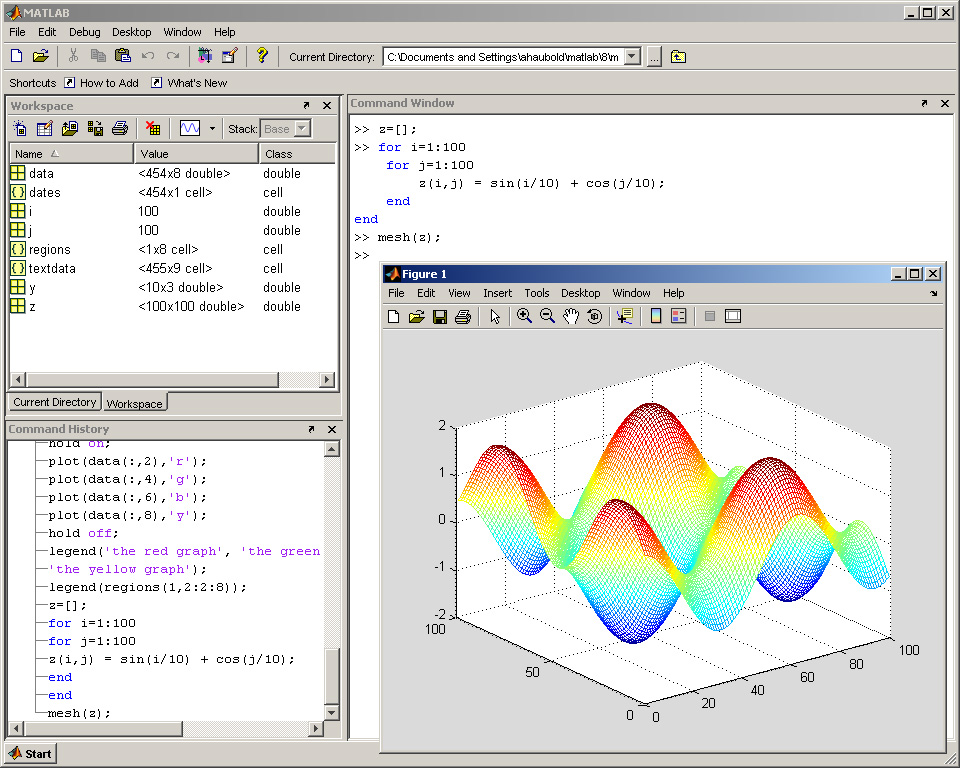
\includegraphics[scale=0.5]{matlab_mesh.jpg}}
    \caption{Capture d'écran de Matlab}
    \label{fig:matlab}
\end{figure}

\subsection{Saisie de texte augmentée}
L'interface utilisateur associée à cette fonctionnalité sera proche de celle proposée par les traitements de texte classiques, comme LibreOffice ou Microsoft Word. Ainsi, l'utilisateur aura à sa disposition une zone de texte qu'il pourra remplir en tapant au clavier. Dans cette zone de texte, il pourra sélectionner du texte avec la souris. Si du texte est sélectionné et qu'il clique sur un bouton de mise en forme, la mise en forme sera effectuée et présentée dans la zone de texte. Cela ressemblerait donc au schéma présenté dans la figure~\ref{fig:saisie_texte_augmentee_UI}.

\begin{figure}[!ht]
	\centerline{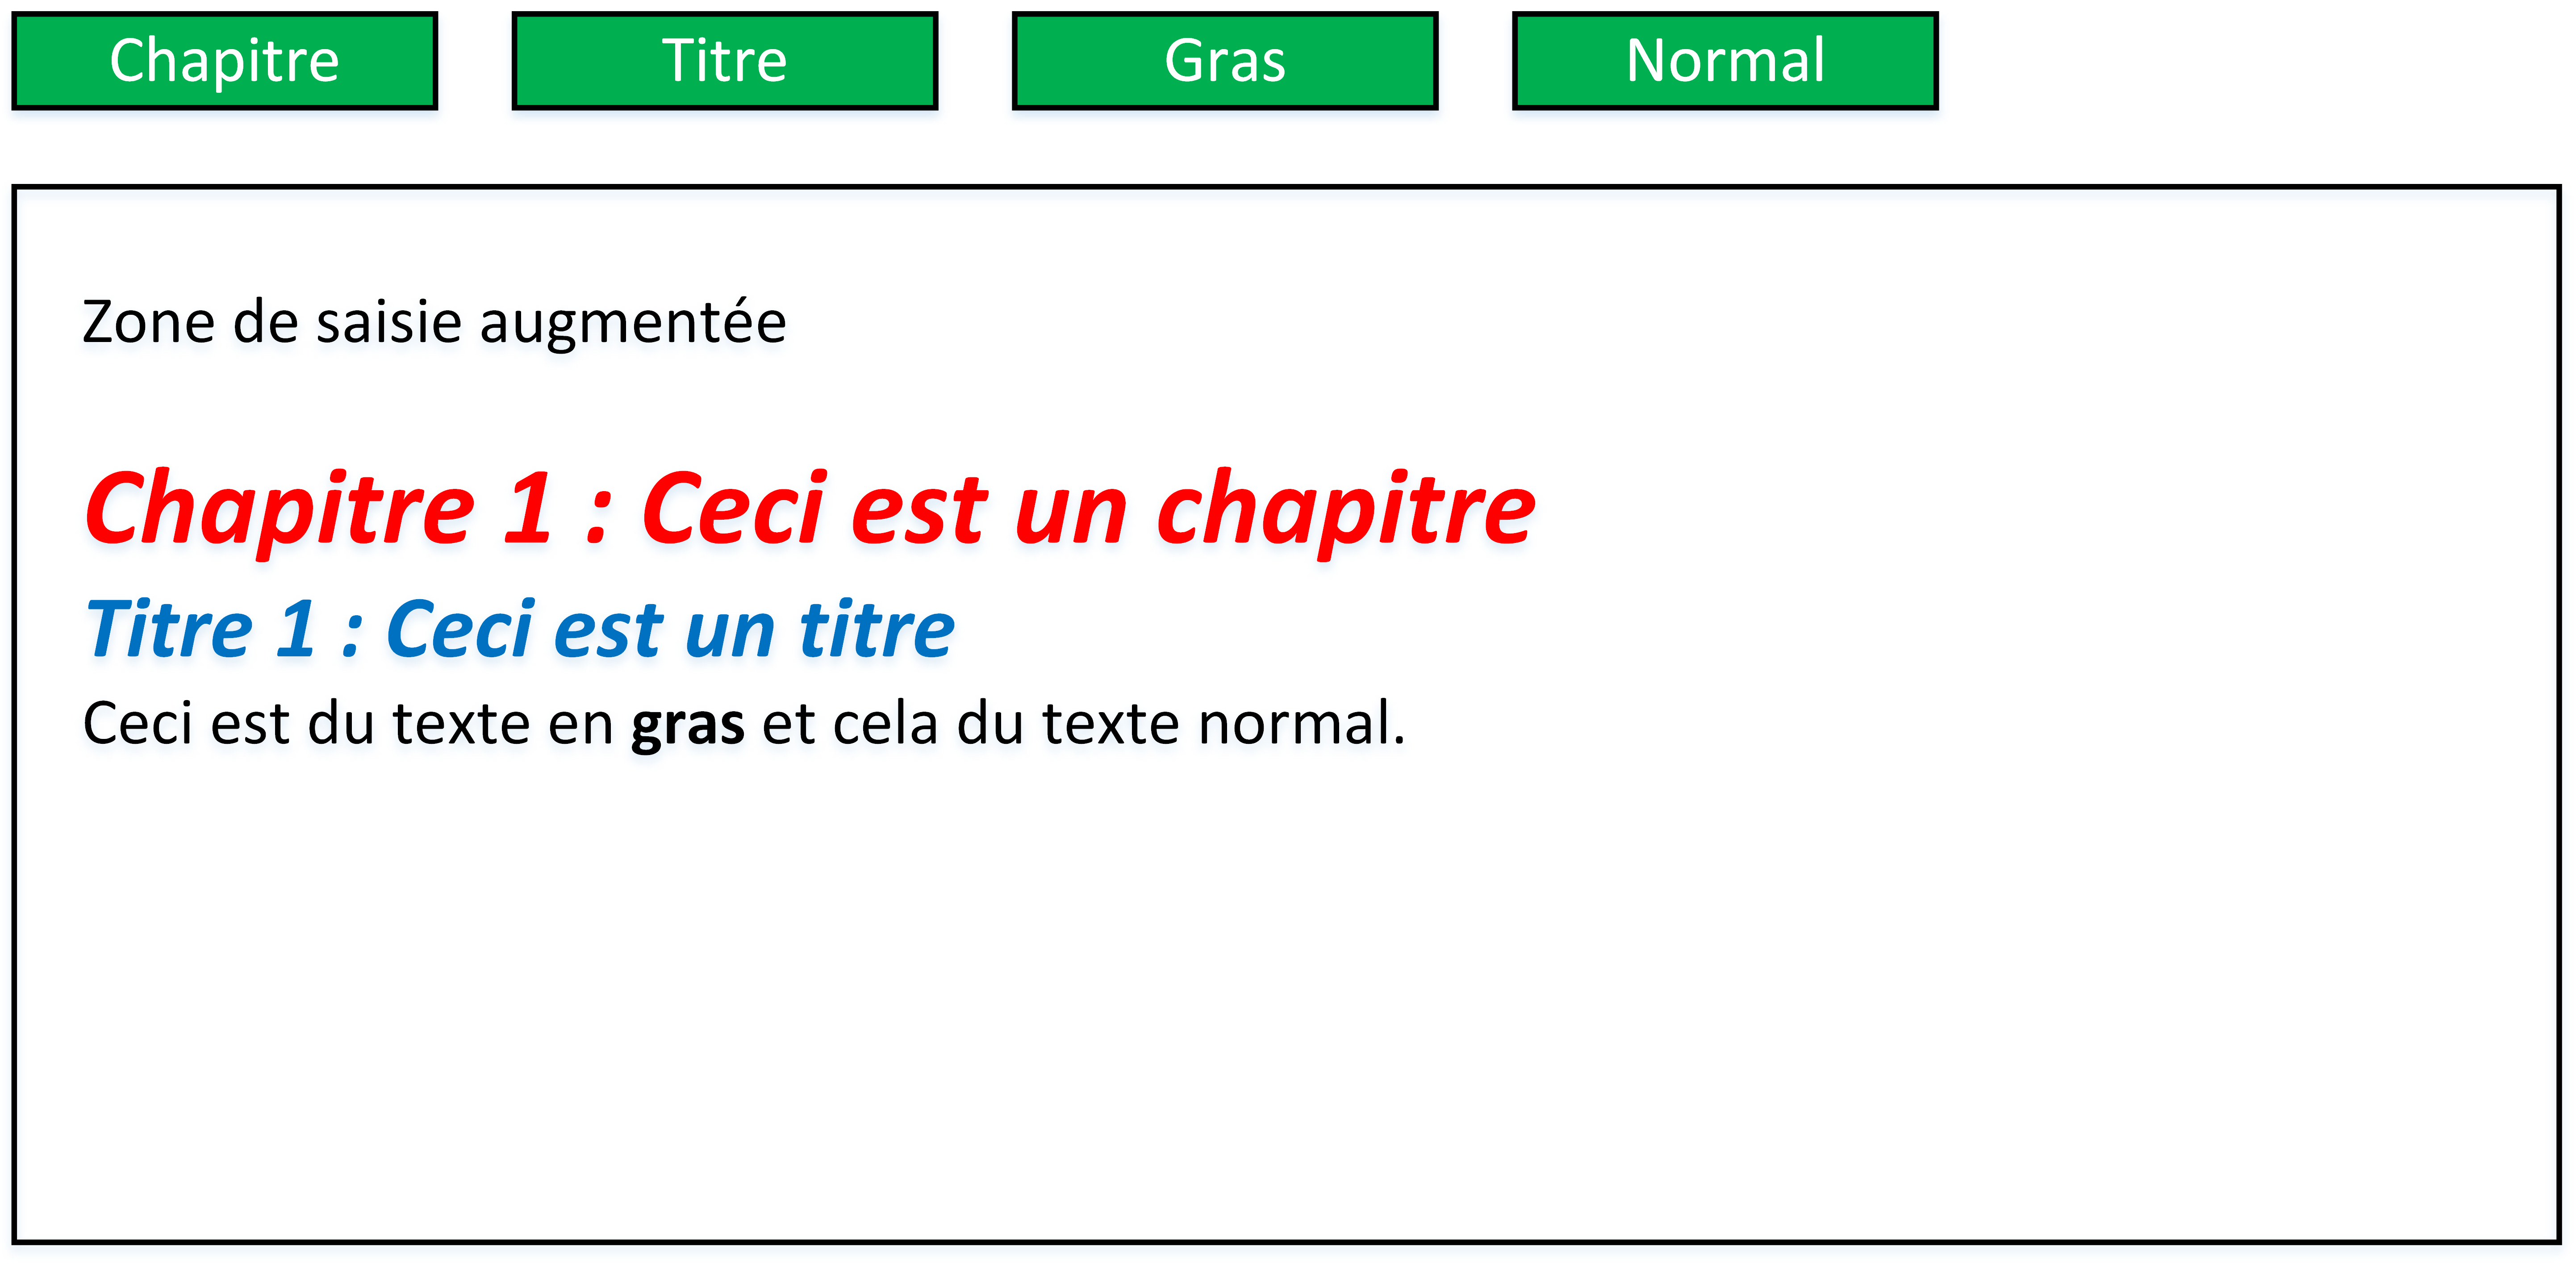
\includegraphics[scale=0.4]{saisie_texte_augmentee.png}}
    \caption{Schéma représentant la saisie de texte augmentée}
    \label{fig:saisie_texte_augmentee_UI}
\end{figure}

Un plus intéressant serait de pouvoir mettre en forme avec des raccourcis clavier~: \verb"CTRL+0" pour un chapitre, \verb"CTRL+1" pour un titre, \verb"CTRL+B" pour mettre en gras, etc.


\subsection{Fiche personnage}
Le but de cette fiche est de regrouper toutes les informations utiles à l'utilisateur sur un personnage. Une fiche vierge s'ouvre lorsque l'utilisateur choisit de créer un nouveau personnage.

La fiche comportera différents champs qui servent à identifier le personnage~:
\begin{itemize}
	\item son nom et son prénom~; 
	\item son teint de peau, ses yeux, ses cheveux~;
	\item son caractère~;
	\item ses relations avec les autres personnages
	\item et les événements dans lesquels il est impliqué.
\end{itemize}

La fiche comportera une option de remplissage aléatoire des champs afin de générer un personnage automatiquement. Dans le cas où l'utilisateur souhaite créer manuellement un personnage ou si la génération aléatoire ne lui convient pas, tous les champs restent modifiables à tout instant. 

Une fois que l'utilisateur a rempli tous les champs qu'il jugeait nécessaire, il pourra valider sa fiche personnage et celle-ci sera enregistrée. A chaque modification, il devra valider à nouveau sa fiche personnage.

L'utilisateur pourra également supprimer un personnage en déplaçant la fiche vers une corbeille.

\subsection{Gestion des liens entre les personnages}
La représentation graphique qui pourrait être adoptée serait la suivante~: le personnage principal serait représenté au centre, avec autour de lui les personnages qui lui sont les plus proches. Plus deux personnages seraient éloignés, moins ils auraient de liens entre eux~; et plus un personnage serait important, plus son image serait grande. En cliquant sur l'avatar d'un personnage, on accéderait à sa fiche détaillée et à la frise restreinte au personnage en question. 

\subsection{Gestion graphique de la frise}
Le but est de rendre l'utilisation de la frise intuitive.

Lorsque l'utilisateur choisit de créer un événement, une fiche événement s'ouvre. Tous les champs à remplir sont optionnels sauf le nom de l'événement qui est impératif pour le placer sur la frise. Une fois les informations remplies, l'utilisateur valide sa saisie. Si une date est saisie, l'événement se place automatiquement sur la frise, sinon, l'utilisateur clique sur l'endroit de la frise où il souhaite ajouter l'événement.

Pour déplacer un événement, il suffira de le faire glisser sur une autre partie de la frise. Une confirmation de déplacement sera demandée. On pourra aussi utiliser le clic droit qui proposera, au choix, de modifier ou supprimer l'événement. Pour supprimer un événement, on pourra soit le faire glisser vers une image de corbeille située en haut à gauche de la fenêtre, soit utiliser le clic droit.

Lorsque l'on clique sur un événement, sa fiche s'ouvre. L'utilisateur peut ainsi modifier toutes les informations relatives à l'événement. Il peut aussi cliquer sur le nom d'un personnage ce qui le renvoie directement à la fiche du personnage.

\subsection{Enregistrement et sauvegarde d'un projet}
L'utilisateur pourra sauvegarder, charger ou créer un projet via un menu \texttt{Fichier}, placé en haut de l'interface utilisateur. Il pourra, en outre, lancer les fonctions de création, sauvegarde et restauration du projet grâce à des raccourcis clavier. On utilisera par exemple le raccourci clavier \verb"CTRL+S" pour enregistrer le projet courant, \verb"CTRL+O" pour ouvrir un projet ou encore \verb"CTRL+N" pour créer un nouveau projet de toute pièce.


%%%%%%%%%%%%%%%%%%%%%%%%%%%%%%%%%%%%%%%%%%%%%%%%%%%%%%%%%%%%%%%%%%%%%%%%%%%%%%%%%%%%%%%%%%%%%%%%%%%%%%%%%%%%%%%%%%%%%%
%%%%%%%%%%%%%%%%%%%%%%%%%%%%%%%%%%%%%%%%%%%%%%%%%%%%%%%%%%%%%%%%%%%%%%%%%%%%%%%%%%%%%%%%%%%%%%%%%%%%%%%%%%%%%%%%%%%%%%
\section*{Annexe~: points nous paraissant complexes}
Après analyse, les points suivants nous paraissent difficiles~:
\begin{itemize}
	\item Affichage du texte mis en forme dans la zone d'édition du manuscrit ;
    \item Réaliser le dictionnaire de ressenti, le problème que nous voyons surtout ici serait pour la création de la base de données de champ lexical par ressentis~;
    \item Utilisation de l'API de LanguageTool pour implanter le correcteur grammatical et orthographique.
\end{itemize}

%====[ FIN DU DOCUMENT ]====================================================
\end{document}